\documentclass[10pt,letterpaper]{article}
\usepackage[margin=.79in,top=.72in,bottom=.72in]{geometry}
\usepackage[T1]{fontenc}
\usepackage{lmodern,microtype}
\usepackage{amsmath,amssymb,amsthm}
\usepackage{graphicx}
\usepackage[hidelinks]{hyperref}
\usepackage{enumitem}
\setlength{\parindent}{0pt}
\setlength{\parskip}{4pt}
\setlist{nosep,leftmargin=*}
\newtheorem{theorem}{Theorem}
\newtheorem{lemma}{Lemma}
\newtheorem{proposition}{Proposition}
\hypersetup{pdftitle={Search Under a Disorder Budget},pdfauthor={Jonathan R. Landers}}
\begin{document}
\begin{center}
{\Large\bfseries Search Under a Disorder Budget}\\[2pt]
{\small Preprocessing, repeated queries, and adaptive indexing}\\[5pt]
Jonathan R. Landers \qquad October 9, 2026
\end{center}

\textbf{Abstract.} A bound on an array's rank-displacement potential limits
single-search cost, but repeated searches can share comparisons spent on the
array itself. We give three choices: search without preprocessing, build a
sorted index from the maximum-displacement certificate, or build one with an
inversion-adaptive sort. The last choice improves the index cost to
$O(n+n\log(1+E/n))$ under a potential promise $V(A)\le E$; an elementary
insertion-sort argument already gives $O(n+E)$. We keep preprocessing and
query comparisons in one accounting model, and distinguish lower bounds for
complete indexing from those for repeated search.

\section{Historical orientation}
The classical comparison model separates two tasks. An unordered array may
require a linear scan for one search, while a sorted array supports binary
search. Producing a sorted index costs $\Theta(n\log n)$ comparisons in the
unrestricted worst case \cite{knuth}. Fredman's work on sorting with prior
information asks how a restricted set of possible orders changes that cost
\cite{fredman}. A disorder promise is one form of such information, provided
the work needed to obtain the promise is not silently omitted.

Mannila treated measures of presortedness as algorithmic resources
\cite{mannila}. In particular, the number of inversions supports adaptive
sorting: Elmasry and Fredman give an $O(n)$-space algorithm using
$n\log_2(1+I/n)+O(n)$ comparisons when the input has $I$ inversions
\cite{elmasryfredman}. On the search side, bounded displacement is a useful
certificate for searching nearly sorted arrays \cite{disser}. The first
paper in this series converts the squared rank-displacement potential into
such a certificate and proves a tight one-query bound \cite{first}.
This note joins those two routes to a reusable sorted index.

\section{Model and the one-query baseline}
Let $A=(a_1,\ldots,a_n)$ contain $n\ge2$ distinct keys from a totally
ordered universe, and let $x_i$ be the sorted rank of $a_i$. Define
\[
 V(A)=\frac12\sum_{i=1}^n(x_i-i)^2,\qquad
 d(A)=\max_i|x_i-i|,\qquad V(A)\le E.
\]
The supplied promise $V(A)\le E$ says nothing about the actual ranks
available to an algorithm. The displacement lemma of \cite{first} gives
\[
 d(A)\le D_E:=
 \min\left\{n-1,\left\lfloor\frac{\sqrt{1+8E}-1}{2}\right\rfloor\right\},
 \qquad R_E=D_E+1.
\]
Indeed, moving one item by $d$ positions requires at least $d$ units of
opposing displacement; hence $2V(A)\ge d^2+d$. Without preprocessing, a
modified binary search followed by a scan uses $O(\log n+R_E)$ target-to-key
comparisons. The matching lower bound in \cite{first} moves a new minimum
past $j-1$ keys at potential $j(j-1)/2$. Thus the one-query minimax cost is
$\Theta(\log n+R_E)$.

Now keep the array fixed for $q\ge1$ searches. Preprocessing may compare
array keys and retain an $O(n)$-word index. Each later query compares its
target with array keys and returns the matching position or absence.
All preprocessing comparisons and target comparisons are charged. With
$\mathcal H_{t-1}$ denoting retained search history, define
\[
 T_q^*(n,E)=\inf_{P,S}
 \sup_{\substack{A:\,V(A)\le E\\y_1,\ldots,y_q}}
 \left[C_P(A)+\sum_{t=1}^q C_S(y_t\mid A,P,\mathcal H_{t-1})\right].
\]
The promise is supplied, as in the first paper. Certifying it from raw
keys would be additional preprocessing work. A complete sorted index is
an array of the original positions in increasing key order; once built,
it supports every search in $O(\log n)$ comparisons.

\section{Potential as a weighted inversion count}
Write $I(A)=|\{(i,j):i<j,\ x_i>x_j\}|$ for the inversion count. The same
potential used for the displacement bound has another exact form.

\begin{lemma}[Weighted inversions]\label{lem:weighted}
For every rank word $x$,
\[
 V(A)=\sum_{\substack{i<j\\x_i>x_j}}(x_i-x_j)\ \ge\ I(A).
\]
\end{lemma}
\begin{proof}
Sort the rank word by swapping adjacent inverted ranks $a>b$. Such a
swap reduces $V$ by exactly $a-b$: the squared-displacement terms at
the two affected positions give this difference directly. An
inversion-removing adjacent-swap sort crosses each originally inverted
pair once and ends with potential zero. Summing its decreases proves
the identity. Every rank gap in the sum is at least one.
\end{proof}

The lemma converts the supplied bound $V(A)\le E$ into $I(A)\le E$.
It does not reveal the inversion locations. It gives an algorithmic
choice because inversion-adaptive sorting needs no advance list of
those locations.

\section{Three preprocessing choices}
\begin{theorem}[Repeated-search upper bound]\label{thm:three}
For $n\ge2$, $E\ge0$, and $q\ge1$ in the model above,
\[
 \boxed{\displaystyle
 T_q^*(n,E)=O\!\left(
 q\log n+\min\left\{
 qR_E,\quad n\log(R_E+1),\quad
 n\bigl[1+\log(1+E/n)\bigr]
 \right\}\right).}
\]
All logarithms are base $2$. If $E=0$, the array is already sorted
and no preprocessing comparisons are needed.
\end{theorem}
\begin{proof}
\textbf{Search directly.} Use the bounded-displacement search for
each target. This spends no preprocessing comparisons and
$O(q\log n+qR_E)$ comparisons in total.

\textbf{Index from displacement.} The key of rank $k$ lies by
position $k+D_E$. Start a min-heap containing positions
$1,\ldots,\min\{n,D_E+1\}$. Extract its minimum and insert the next
unread position, repeating until all keys are output. Before the
$k$th extraction, the heap contains every unread key among the first
$\min\{n,k+D_E\}$ positions, including rank $k$. It therefore emits
the sorted order using a heap of size at most $R_E$. This costs
$O(n\log(R_E+1))$ array-key comparisons and $O(n)$ words. Search the
resulting index by binary search for another $O(q\log n)$ comparisons.

\textbf{Index from inversions.} First, a self-contained weaker choice
is ordinary insertion sort applied to an array of positions. Each
successful backward comparison removes one inversion, and there is
at most one stopping comparison per inserted key. It uses at most
$I(A)+n-1\le E+n-1$ array-key comparisons and $O(n)$ words. The
inversion-adaptive algorithm of Elmasry and Fredman
\cite{elmasryfredman} strengthens this to
$n\log(1+I(A)/n)+O(n)$ comparisons using $O(n)$ space; it does not
need to know $I(A)$ beforehand. Lemma~\ref{lem:weighted} bounds this
by $n\log(1+E/n)+O(n)$. Retain the resulting sorted positions and
binary-search them for the $q$ targets. Choosing the cheapest of the
three strategies proves the theorem.
\end{proof}

The third branch matters when total disorder is small but the largest
possible displacement is not. For example, if $E=\Theta(n)$, then
$R_E=\Theta(\sqrt n)$. The heap branch can spend
$\Theta(n\log n)$ comparisons building an index, while adaptive
sorting spends $O(n)$. The crossover against repeated direct search
is then $qR_E\asymp n$, up to constants. For large $E$, either
indexing method may cost $\Theta(n\log n)$; the minimum retains both.
The theorem is an upper bound on the combined problem, not a claim
that each of its three terms is necessary.

\section{Regimes and examples}
The new branch has the strongest effect before the scalar displacement
certificate saturates. Compare the index-construction expressions
\[
 B_{\mathrm{disp}}(n,E)=O(n\log(R_E+1)),\qquad
 B_{\mathrm{inv}}(n,E)=O\!\left(n\left[1+\log(1+E/n)\right]\right).
\]
For $E=0$, the promise itself identifies sorted order. For
$1\le E=O(n)$, the inversion branch costs $O(n)$, while the
heap expression may grow to $\Theta(n\log n)$ as $E$ approaches $n$.
For $n\ll E\ll n^2$, the adaptive logarithm depends on $E/n$;
the heap logarithm depends on roughly $\sqrt E$. When
$E\ge n(n-1)/2$, the displacement certificate has saturated at
$R_E=n$, and the heap uses $O(n\log n)$ comparisons. The
inversion branch also gives at most $O(n\log n)$ because no
permutation has more than $\binom n2$ inversions. These statements
compare construction guarantees; the theorem chooses between
constructing an index and searching directly for a given $q$.

Two small families clarify what the potential does and does not reveal.
First, swap $k$ disjoint adjacent pairs in an otherwise sorted array.
Then $V=I=k$ and $d=1$. A supplied scalar budget $E=k$ allows much
larger displacement on other arrays, so the one-query worst-case
search cost still depends on $R_E$; a full index can be built in
$O(n)$ comparisons when $k=O(n)$. Second, move the minimum from
position $j$ to position $1$ while shifting the preceding $j-1$
items right. Then
\[
 V=\frac{j(j-1)}2,\qquad I=j-1,\qquad d=j-1.
\]
This input attains the displacement obstruction behind the first
paper's search lower bound, yet its inversion count is only linear
in $j$. An inversion-adaptive sorter takes $O(n)$ comparisons on
this particular input, even when the general bound based on its
potential budget is larger. The reverse permutation provides the
opposite scale: $V=n(n^2-1)/6$ and $I=n(n-1)/2$, so both full-index
strategies have the familiar $O(n\log n)$ guarantee.

The exact $n=9$ histogram below illustrates where a tight scalar budget
still narrows the displacement window. Here
$E_{\mathrm{sat}}=n(n-1)/2=36$: a promise $E=V(A)<36$ gives $R_E<n$.
Exactly $48{,}913$ of the $362{,}880$ uniform permutations, or $13.5\%$,
fall in that low-potential tail. This is a coverage calculation, not a
certificate for an unknown input. More generally, a uniform shuffle
typically has $V=\Theta(n^3)$, beyond the $\Theta(n^2)$ saturation scale
\cite{permutation}. The improved preprocessing bound is therefore most
informative for input classes that favor near-sorted order. It remains
a worst-case guarantee for every array covered by its stated budget.

\begin{figure}[htbp]
\centering
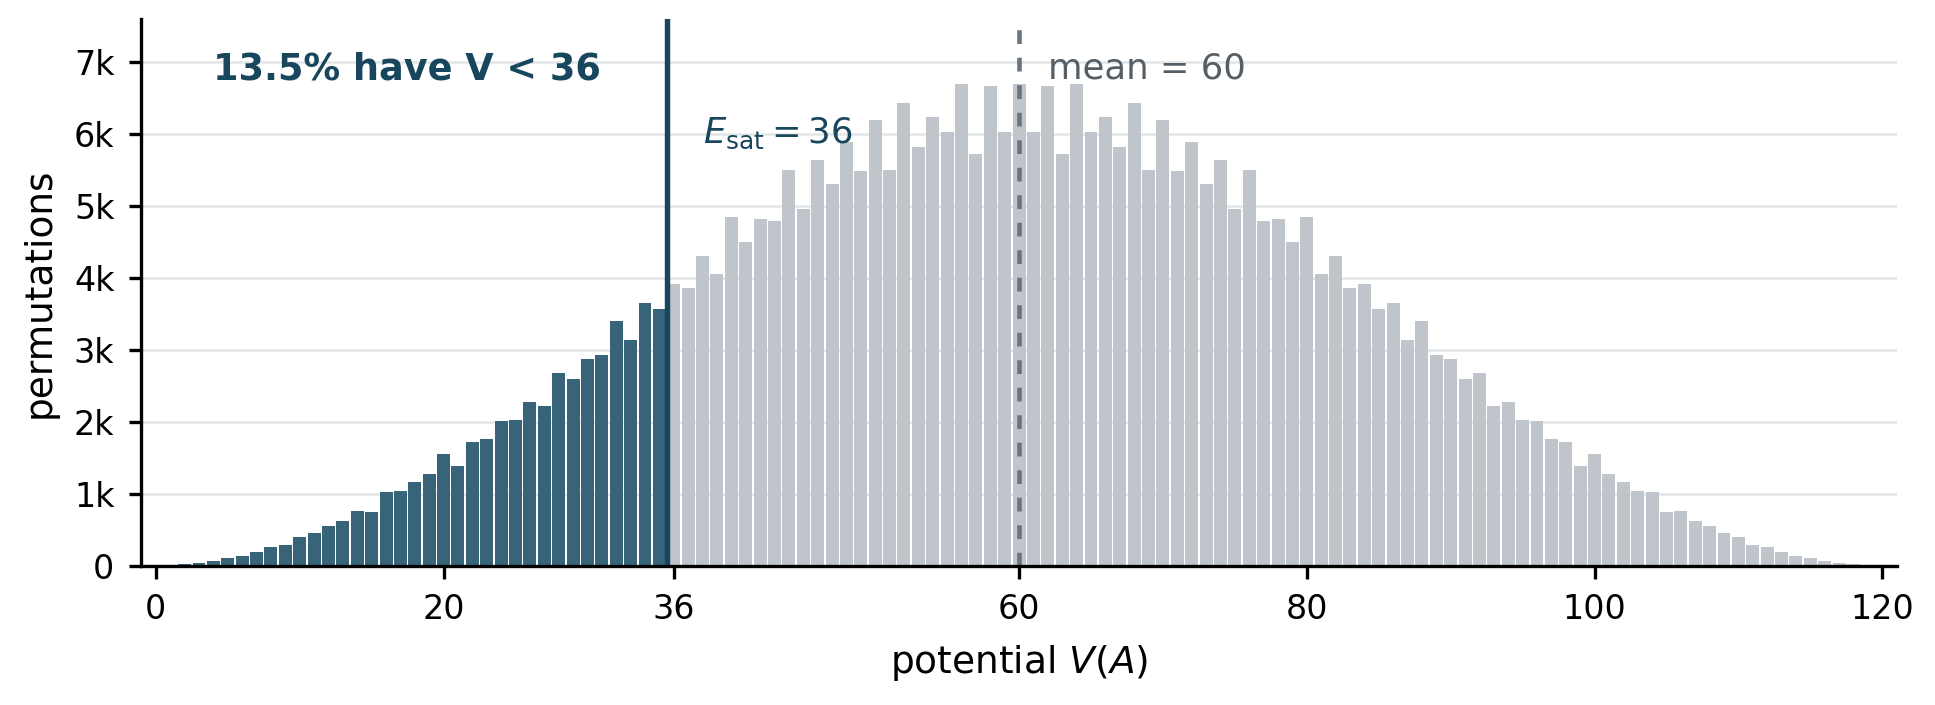
\includegraphics[width=.96\linewidth]{potential_budget_n9.png}
\caption{Exact counts for all 362,880 permutations of nine ranks.
Dark bars mark the 48,913 permutations (13.5 percent) with potential
below 36, the saturation threshold for the displacement certificate
under a tight budget. The dashed line marks the mean potential 60.}
\label{fig:budget}
\end{figure}

\section{What lower bounds do and do not say}
The full sorted-index task has a simple linear obstruction whenever
$E\ge1$. On a sorted input, swap the keys at any adjacent pair of
positions. Each alternative has potential one. Every comparison
except that pair's direct comparison has the same outcome as on the
sorted input. A method that must output the entire sorted index
therefore compares all $n-1$ adjacent pairs on the sorted input.
Consequently, full indexing requires $\Omega(n)$ comparisons for
$E\ge1$, and the inversion-adaptive branch is optimal up to constants
for that task when $E=O(n)$.

Exact potential counts offer another, weaker, information bound.
If $c_n(v)$ is the number of rank words with potential $v$, put
$N_{n,E}=\sum_{v\le E}c_n(v)$. A comparison tree that outputs a full
sorted index for every promised rank word needs at least
$\lceil\log_2N_{n,E}\rceil$ comparisons in the worst case. The
random-permutation histogram gives these counts exactly for $n=9$,
including its small parity oscillations. Neither this count nor the
linear indexing obstruction automatically lower-bounds $T_q^*$:
an optimal repeated-search method may build only part of an index.
The smallest nonzero budget shows why cardinality alone is incomplete.
At $E=1$, the bound $\sum_i(x_i-i)^2\le2$ forces either zero
displacement or two opposite unit displacements. The only allowed rank
words are therefore the sorted order and its $n-1$ possible adjacent
swaps, so $N_{n,1}=n$. Its information bound
is merely $\lceil\log_2 n\rceil$, while the adjacent-pair adversary
above forces $n-1$ comparisons to output the complete index on the
sorted input. The arrangement of feasible orders matters as well as
their number.

There is a separate lower bound when history retains only prior
target-to-entry signs and no array-key comparisons are allowed. Run
the searcher on a sorted array with increasing absent targets
$y_1<\cdots<y_q<a_1$. In round $t$, replacing position
$j\le R_E$ by $y_t$ gives an allowed array of potential
$j(j-1)/2$. Earlier targets remain below every entry in both
arrays. Unless the searcher checks position $j$ in that round, its
comparison signs match the sorted case despite a different correct
answer. Thus all first $R_E$ positions must be checked each round,
for $\Omega(qR_E)$ target comparisons in this restricted model.
Array-key preprocessing can escape this argument; it is precisely
what the two index strategies pay for.

\newpage
\section{Certificates and scope}
A learned rule may propose a smaller displacement bound, likely key
locations, or a partial index. Only a verified guarantee can be used
for worst-case correctness. If $B$ array-key comparisons certify
$d(A)\le D'$, the first paper's search gives
\[
 \text{total cost}\le B+O\!\left(q\log n+q(D'+1)\right).
\]
For example, checking all $n-1$ adjacent pairs certifies sortedness.
This is worthwhile only when enough later searches use that fact.
A full sorted index also reveals every actual rank, and hence the
actual displacement, without further key comparisons once it is
built. At that point the index itself supports binary search; a
separate displacement certificate adds no search power. The
interesting intermediate case is a cheaper partial certificate that
reduces the residual scan before all ranks have been learned.
The comparisons used to obtain a smaller certificate belong in $B$.
A mere prediction of $D'<D_E$ is not valid over every input allowed
by $V(A)\le E$: some such inputs attain $D_E$.

The refined upper bound shows two ways that the same potential promise
can subsidize an index. Its maximum-displacement consequence powers
the heap; its weighted-inversion consequence powers adaptive sorting.
The exact distribution of potential across random permutations
describes how often a budget covers an input, while the theorem holds
for every array covered by that budget. A matching lower bound for
the full preprocessing-versus-query tradeoff remains open here.
The theorem compares one strategy with no array comparisons and two
strategies that build a complete sorted index. It does not rule out
partial preprocessing that lies between those endpoints. Such a
result would need a lower-bound model that tracks what array
comparisons reveal about future target locations, as well as an
algorithm that charges every comparison used to obtain its
certificate. Exact level-set counts are useful input for that study,
but cannot by themselves certify the cost of a search strategy.

{\footnotesize
\begin{thebibliography}{9}
\bibitem{knuth} D. E. Knuth. \emph{The Art of Computer Programming,
Volume 3: Sorting and Searching}. Addison-Wesley, 1973; 2nd ed., 1998.
\href{https://cs.stanford.edu/~knuth/taocp.html}{Author's publication page}.
\bibitem{fredman} M. L. Fredman. How good is the information theory
bound in sorting? \emph{Theoretical Computer Science} 1(4):355--361,
1976. \href{https://doi.org/10.1016/0304-3975(76)90078-5}
{doi:10.1016/0304-3975(76)90078-5}.
\bibitem{mannila} H. Mannila. Measures of presortedness and optimal
sorting algorithms. \emph{IEEE Transactions on Computers}
C-34(4):318--325, 1985.
\href{https://doi.org/10.1109/TC.1985.5009382}{doi:10.1109/TC.1985.5009382}.
\bibitem{disser} Y. Disser and S. Kratsch. Robust and adaptive search.
STACS 2017, LIPIcs 66, 26:1--26:14.
\href{https://doi.org/10.4230/LIPIcs.STACS.2017.26}
{doi:10.4230/LIPIcs.STACS.2017.26}.
\bibitem{elmasryfredman} A. Elmasry and M. L. Fredman. Adaptive sorting:
an information theoretic perspective. \emph{Acta Informatica}
45:33--42, 2008.
\href{https://doi.org/10.1007/s00236-007-0061-0}
{doi:10.1007/s00236-007-0061-0}.
\bibitem{first} J. R. Landers. \emph{Disorder Potential and the Cost of
Search}, version 2, 2026.
\href{https://jonland82.github.io/algorithmic-search-cost/disorder_potential_search_note_v2.html}
{HTML edition}.
\bibitem{permutation} J. R. Landers. \emph{Potential Across Random
Permutations}, companion note, 2026.
\href{https://jonland82.github.io/algorithmic-search-cost/experiments/n9-potential-distribution/potential_across_random_permutations.html}
{HTML edition}.
\end{thebibliography}
}
\end{document}
